\documentclass[30pt,twocolumn,letterpaper]{article}
\usepackage{cvpr}
\usepackage{times}
\usepackage{booktabs}
\usepackage{epsfig}
\usepackage{graphicx}
\usepackage{amsmath}
\usepackage{amssymb}
\cvprfinalcopy
\def\cvprPaperID{****}
\def\httilde{\mbox{\tt\raisebox{-.5ex}{\symbol{126}}}}
\usepackage{graphicx}
\usepackage{indentfirst}
\setlength{\parindent}{2em}
\usepackage{cite}
\usepackage[colorlinks,linkcolor=red,anchorcolor=blue,citecolor=green,backref=page]{hyperref}
\author{Qilei Zhang\\\\
Jul 8 2018}
\title{Supervised Discrete Hashing}
\begin{document}
\maketitle
\begin{abstract}
  Recently, learning based hashing techniques have attracted broad research interests because they can support efficient storage and retrieval for high-dimensional data such as images, videos, documents, etc. However, a major difficulty of learning to hash lies in handling the discrete constraints imposed on the pursued hash codes, which typically makes hash optimizations very challenging.
\end{abstract}
\section{Introduction}
Hashing has attracted considerable attention of researchers in computer vision, machine learning, information retrieval and related areas. Hashing techniques encode documents, images, videos or other sorts of data by a set of short binary codes, while preserving the similarity of the original data\cite{Gupta2014Biperpedia}. With the binary codes, the task of nearest neighbour search can be easily conducted on large-scale dataset, due to the high efficiency of pairwise comparison with the Hamming distance\cite{Li2017Kernelised}. \\
\begin{figure}[htbp]
\small
\centering
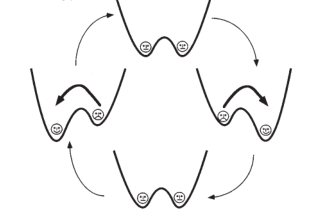
\includegraphics[width=20em]{000.png}
\caption{Results of the compared methods in precision of Hamming distance 2 and MAP on CIFAR-10 with code length from 16 to 128.}
\label{fig:lable}
\end{figure}\\
\section{Experiments}
Extensive experiments were carried out to assess the computational efficiency and retrieval performance of the proposed hash method. Test in four large image data sets. All data samples are normalized to unit length. Compared with several state-of-the-art supervised hashing methods\cite{Mukhtarov2014New}.\\
\begin{figure}[htbp]
\small
\centering
\includegraphics[width=20em]{001.png}
\caption{Results of the compared methods in precision and recall of Hamming distance 2 on MNIST with code length from 16 to 128.}
\label{fig:lable}
\end{figure}\\
\section{Conclusion}
Reexamine the issue of a supervised hash. In order to make full use of semantic label information, a joint learning objective is formulated, which integrates hash code generation and linear classifier training. When the target is optimized, the generated hash code is expected to be the best classifier for joint training\cite{Yao2013Semi}.\\
{\small
\bibliographystyle{ieee}
\bibliography{1}
}
\end{document}
